% BUBBLE-BLUE, NetMob 2026 talk. ~30 minutes, 16:9.
% Compile: pdflatex twice.
% Suggested pace is in the comments after each \section.
\documentclass[aspectratio=169,11pt]{beamer}
\usetheme{default}
\usecolortheme{default}
\setbeamertemplate{navigation symbols}{}
\setbeamertemplate{footline}{%
  \hspace{3.5mm}{\tiny\color{muted}NetMob 2026 \textperiodcentered{} Niterói}%
  \hfill{\tiny\color{muted}\insertframenumber/\inserttotalframenumber}\hspace{3.5mm}\vspace{2.2mm}}
\setbeamertemplate{itemize item}{\color{accent}\textbullet}
\setbeamertemplate{itemize subitem}{\color{navy}\textendash}
\setbeamertemplate{enumerate item}{\color{accent}\insertenumlabel.}
\setbeamerfont{frametitle}{series=\bfseries,size=\large}
\setbeamercolor{frametitle}{fg=navy}
\setbeamercolor{normal text}{fg=ink}
\setbeamercolor{structure}{fg=navy}
\setbeamercolor{math text}{fg=ink}
\setbeamercolor{block title}{fg=navy, bg=scr}
\setbeamercolor{block body}{fg=ink, bg=hdr}
\setbeamertemplate{blocks}[rounded][shadow=false]

\usepackage[T1]{fontenc}
\usepackage{lmodern}
\usepackage{tgheros}
\renewcommand{\familydefault}{\sfdefault}
\usepackage{amsmath,amssymb}
\usepackage{booktabs}
\usepackage{tikz}
\usetikzlibrary{positioning,calc,fit,decorations.pathreplacing}
\usepackage{pgfplots}
\pgfplotsset{compat=1.17}

\definecolor{navy}{HTML}{14213D}
\definecolor{accent}{HTML}{C8102E}
\definecolor{ink}{HTML}{1F2937}
\definecolor{muted}{HTML}{5B6472}
\definecolor{scr}{HTML}{DCE6F5}
\definecolor{rel}{HTML}{DCEFE3}
\definecolor{hdr}{HTML}{EEF0F3}

\newcommand{\figcap}[1]{\par\vspace{1mm}{\scriptsize\color{muted}#1\par}}
\newcommand{\metric}[2]{%
  \begin{minipage}[t]{0.30\linewidth}\centering
  {\color{accent}\bfseries\Large #1}\\[1mm]{\scriptsize #2}
  \end{minipage}}

\title{BUBBLE-BLUE}
\subtitle{Private group messaging over an open Bluetooth LE mesh}
\author{Paul-Maxence Baraton$^1$ \and Nadjib Achir$^1$ \and Philippe Jacquet$^1$ \and Wilfred Doré$^2$}
\institute{$^1$Inria, France \qquad $^2$Qualcomm, France}
\date{NetMob 2026 \textperiodcentered{} Niterói}

\begin{document}

% =====================================================================
% 0--2 min  title and plan
% =====================================================================
\begin{frame}[plain]
\begin{tikzpicture}[remember picture, overlay]
  \fill[navy] (current page.south west) rectangle (current page.north east);
  \fill[accent] ([yshift=11mm]current page.south west) rectangle ([yshift=12.2mm]current page.south east);
\end{tikzpicture}
\vspace{8mm}
{\color{white}\bfseries\Huge BUBBLE-BLUE\par}
\vspace{4mm}
{\color{white!85}\Large Private group messaging\\over an open Bluetooth LE mesh\par}
\vspace{10mm}
{\color{white}Paul-Maxence Baraton, Nadjib Achir, Philippe Jacquet \textcolor{white!70}{(Inria)}\\
Wilfred Doré \textcolor{white!70}{(Qualcomm)}\par}
\vspace{6mm}
{\color{white!65}NetMob 2026 \textperiodcentered{} Niterói \qquad arXiv:2509.00967}
\end{frame}

\begin{frame}{30 minutes}
\begin{enumerate}
  \item Why an open mesh with a private group
  \item How a frame travels, and who is allowed to read it
  \item How two members share a key, and how we drop one
  \item What six boards measured: a room, a building, a working day
  \item What broke, what we do not claim, what comes next
\end{enumerate}
\vspace{6mm}
{\color{muted}\small The stand is next to the poster: send, exclude, restart.}
\end{frame}

% =====================================================================
% 2--7 min  idea
% =====================================================================
\begin{frame}{The settings that need this}
Local communication still collapses onto a Wi-Fi access point, or onto a
phone OS that will not host a third-party mesh.
\vspace{4mm}
\begin{itemize}
  \item a crowd at an event: the infrastructure is saturated
  \item a site without coverage
  \item an emergency response: the infrastructure is absent or distrusted
\end{itemize}
\vspace{5mm}
Bluetooth is on every device and needs no operator.\\[2mm]
The question is not ``can two phones see each other''.\\
It is: \textbf{can a stranger carry a conversation they will never read?}
\end{frame}

\begin{frame}{Two things existing meshes merge}
\begin{columns}[T,onlytextwidth]
\begin{column}{0.48\textwidth}
\begin{block}{The mesh (open)}
any board may join and relay,\\
including traffic it cannot decrypt.\\[2mm]
{\small no pairing, no bond}
\end{block}
\end{column}
\begin{column}{0.48\textwidth}
\begin{block}{The bubble (private)}
a group exists only for the holders of a key.\\[2mm]
{\small membership is cryptographic,\\not a Bluetooth relationship}
\end{block}
\end{column}
\end{columns}
\vspace{8mm}
\centering
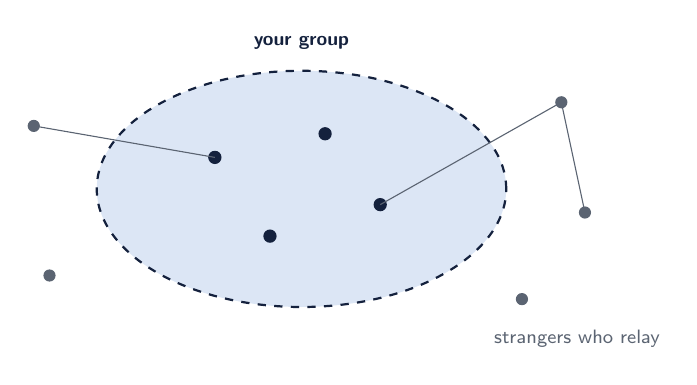
\begin{tikzpicture}[font=\small]
  \fill[scr, rounded corners=3mm] (0,0) ellipse (2.6 and 1.5);
  \draw[navy, dashed, thick] (0,0) ellipse (2.6 and 1.5);
  \foreach \p in {(-1.1,0.4),(0.3,0.7),(1.0,-0.2),(-0.4,-0.6)}
    \fill[navy] \p circle (2.4pt);
  \node[font=\scriptsize\bfseries, navy] at (0,1.85) {your group};
  \foreach \p in {(3.3,1.1),(3.6,-0.3),(2.8,-1.4),(-3.2,-1.1),(-3.4,0.8)}
    \fill[muted] \p circle (2.2pt);
  \draw[muted] (1.0,-0.2) -- (3.3,1.1) -- (3.6,-0.3);
  \draw[muted] (-1.1,0.4) -- (-3.4,0.8);
  \node[font=\scriptsize, muted] at (3.5,-1.9) {strangers who relay};
\end{tikzpicture}
\end{frame}

\begin{frame}{Where BUBBLE-BLUE sits}
{\small
\begin{tabular}{@{}lccc@{}}
\toprule
System & Data plane & Backbone & Open relay \\
\midrule
SIG Mesh & managed flood & provisioned & no \\
BitChat & GATT flood & none & n/a \\
Briar & RFCOMM, Wi-Fi, Tor & contacts & no \\
Reticulum & multi-transport & identities & no \\
\textbf{BUBBLE-BLUE} & \textbf{LE CoC} & \textbf{elected CDS} & \textbf{yes} \\
\bottomrule
\end{tabular}}
\vspace{6mm}
\begin{itemize}
  \item SIG Mesh: a relay must hold the network key
  \item BitChat, Bridgefy: a crowd-scale BLE flood, no elected backbone
  \item Briar: only pre-paired contacts
\end{itemize}
\vspace{3mm}
{\color{muted}\small None of the others lets a node sit in an elected backbone
and relay for a group it does not belong to.}
\end{frame}

\begin{frame}{What this talk adds}
The original note gave the algorithms and unit-disk simulations.
\vspace{4mm}
This work:
\begin{enumerate}
  \item a BLE transport (L2CAP connection-oriented channels, no pairing)
  \item a 26-byte frame and a revocation protocol that reaches several hops
  \item measurements on six Qualcomm boards, in a room and across a building
\end{enumerate}
\vspace{6mm}
Not a new routing theory.\\
A protocol that runs on hardware you can pick up.
\end{frame}

% =====================================================================
% 7--14 min  design
% =====================================================================
\begin{frame}{Links without pairing}
A node advertises a compact presence record:
\begin{itemize}
  \item an anonymous identifier
  \item a relay flag
  \item the address at which it accepts connections
\end{itemize}
\vspace{3mm}
Neighbours open an L2CAP CoC at security level \emph{low}:
\textbf{no pairing, no bond, no allow-list}.
\vspace{4mm}
\begin{itemize}
  \item Company ID \texttt{0xFFFF}: the SIG test value (this is a prototype)
  \item HELLO every 5\,s; a neighbour silent for 15\,s is dropped
  \item membership is a 32-byte group key, not a Bluetooth relationship
\end{itemize}
\end{frame}

\begin{frame}{One frame, two planes}
\centering
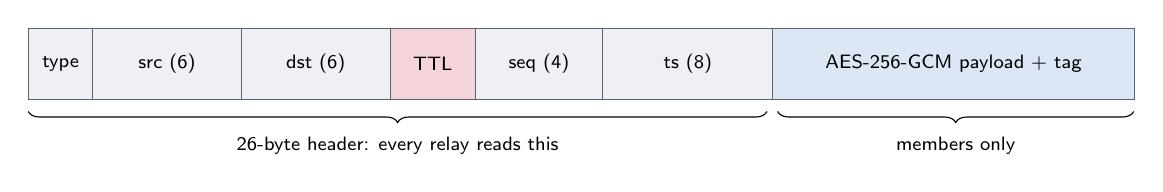
\begin{tikzpicture}[font=\scriptsize, x=1.35mm, y=1mm,
  f/.style={draw=muted, minimum height=9mm, inner sep=0pt, anchor=south west}]
  \foreach \x/\w/\t/\c in {0/6/type/hdr, 6/14/src (6)/hdr, 20/14/dst (6)/hdr,
                           34/8/TTL/accent!18, 42/12/seq (4)/hdr, 54/16/ts (8)/hdr}
    \node[f, fill=\c, minimum width=\w*1.35mm] at (\x,0) {\t};
  \node[f, fill=scr, minimum width=34*1.35mm] at (70,0) {AES-256-GCM payload + tag};
  \draw[decorate, decoration={brace, amplitude=4pt, mirror}] (0,-1.5) -- (69.5,-1.5)
    node[midway, below=2mm] {26-byte header: every relay reads this};
  \draw[decorate, decoration={brace, amplitude=4pt, mirror}] (70.5,-1.5) -- (104,-1.5)
    node[midway, below=2mm] {members only};
\end{tikzpicture}
\vspace{8mm}
\begin{itemize}
  \item relays decrement TTL and forward; they never see the text
  \item header authenticated as associated data, \textbf{except TTL}
  \item up to 470 bytes in one frame
\end{itemize}
\end{frame}

\begin{frame}{Who relays: an elected backbone}
BLE has no native broadcast on a connection.\\
Every local flood is a sequence of unicasts, so flooding everyone is expensive.
\vspace{5mm}
\begin{columns}[T,onlytextwidth]
\begin{column}{0.52\textwidth}
Each node applies the Wu--Li rule to its two-hop view:
\begin{itemize}
  \item marked nodes form a connected dominating set
  \item only they rebroadcast
  \item duplicates dropped on (source, sequence)
\end{itemize}
\vspace{3mm}
{\small The backbone adds no path stretch.\\
Default TTL\,10 spans about twenty nodes (simulation).}
\end{column}
\begin{column}{0.46\textwidth}
\centering
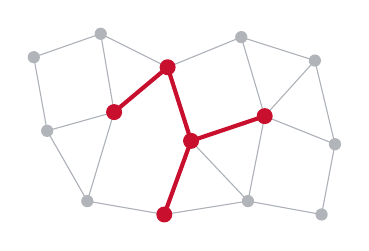
\begin{tikzpicture}[scale=0.85]
  \coordinate (g1) at (-2.2,1.1); \coordinate (g2) at (-1.2,1.45);
  \coordinate (g3) at (-0.2,0.95); \coordinate (g4) at (0.9,1.4);
  \coordinate (g5) at (2.0,1.05); \coordinate (g6) at (-2.0,0.0);
  \coordinate (g7) at (-1.0,0.28); \coordinate (g8) at (0.15,-0.15);
  \coordinate (g9) at (1.25,0.22); \coordinate (g10) at (2.3,-0.2);
  \coordinate (g11) at (-1.4,-1.05); \coordinate (g12) at (-0.25,-1.25);
  \coordinate (g13) at (1.0,-1.05); \coordinate (g14) at (2.1,-1.25);
  \foreach \a/\b in {g1/g2,g2/g3,g3/g4,g4/g5,g1/g6,g6/g7,g2/g7,g7/g3,g3/g8,g8/g9,g4/g9,g9/g5,
                     g9/g10,g5/g10,g6/g11,g7/g11,g11/g12,g8/g12,g12/g13,g8/g13,g13/g14,g10/g14,g9/g13}
    \draw[muted!50] (\a)--(\b);
  \foreach \a/\b in {g7/g3,g3/g8,g8/g9,g8/g12}
    \draw[accent, line width=1.5pt] (\a)--(\b);
  \foreach \n in {g1,g2,g4,g5,g6,g10,g11,g13,g14}
    \fill[ink!35] (\n) circle (2.6pt);
  \foreach \n in {g3,g7,g8,g9,g12}
    \fill[accent] (\n) circle (3.4pt);
\end{tikzpicture}
{\scriptsize\color{muted}backbone, elected locally}
\end{column}
\end{columns}
\end{frame}

\begin{frame}{Group traffic}
With $K_e$ the group key of epoch $e$, every frame gets its own key:
\begin{gather*}
K_{\mathrm{pkt}} = \mathrm{HKDF}(K_e;\ \mathit{src}\,\|\,\mathit{seq}\,\|\,\mathit{ts})\\[2mm]
c = \mathrm{GCM}_{K_{\mathrm{pkt}}}(m;\ \mathit{header})
\end{gather*}
\begin{itemize}
  \item a zero GCM nonce is never reused under one key
  \item a relay without $K_e$ can forward; it cannot read or forge
  \item AES-256-GCM on these boards: 30k--173k pkt/s --- far above the link
\end{itemize}
\vspace{3mm}
{\color{muted}\small The bottleneck is the Bluetooth stack, not the cryptography.}
\end{frame}

% =====================================================================
% 14--21 min  security
% =====================================================================
\begin{frame}{Peer to peer inside the group}
Each board $A$ holds an X25519 secret $a$.\\
Every 30\,s it floods a signed ANNOUNCE binding its address to $A=aG$.
\vspace{3mm}
Two members then share a key without ever having met:
\[
K_{AB}^{(e)} = \mathrm{HKDF}(aB,\ e) = \mathrm{HKDF}(bA,\ e)
\qquad\text{since } aB=bA=abG
\]
\centering
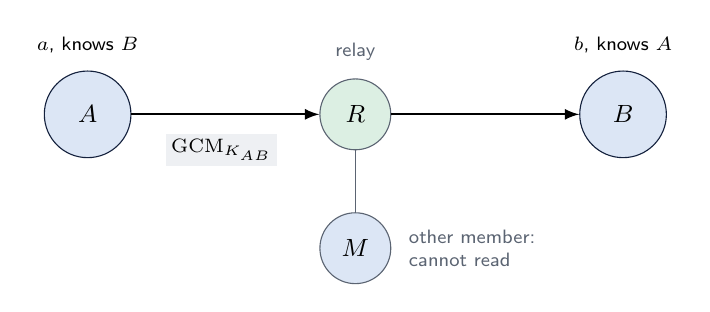
\begin{tikzpicture}[font=\small]
  \node[circle, draw=navy, fill=scr, minimum size=11mm] (a) at (0,0) {$A$};
  \node[circle, draw=muted, fill=rel, minimum size=9mm] (r) at (3.4,0) {$R$};
  \node[circle, draw=navy, fill=scr, minimum size=11mm] (b) at (6.8,0) {$B$};
  \node[circle, draw=muted, fill=scr, minimum size=9mm] (m) at (3.4,-1.7) {$M$};
  \draw[-latex, thick] (a)--(r); \draw[-latex, thick] (r)--(b);
  \draw[muted] (r)--(m);
  \node[above=1mm of a, font=\scriptsize] {$a$, knows $B$};
  \node[above=1mm of b, font=\scriptsize] {$b$, knows $A$};
  \node[above=1mm of r, font=\scriptsize, muted] {relay};
  \node[right=1mm of m, font=\scriptsize, muted, align=left] {other member:\\cannot read};
  \node[font=\scriptsize, fill=hdr, inner sep=2pt] at (1.7,-0.45) {$\mathrm{GCM}_{K_{AB}}$};
\end{tikzpicture}
\figcap{A direct message crosses the mesh like any frame. Relays and other
members forward it; they cannot read it.}
\end{frame}

\begin{frame}{Removing a member $V$}
The coordinator $C$ (smallest anonymous identifier) draws $K_{e+1}$ and a
one-time key $k$, then floods one frame. Each remaining member $i$ gets
$k$ wrapped under the pairwise key it shares with $C$:
\begin{gather*}
w_i = \mathrm{HKDF}(K_{Ci}^{(e)};\ \mathit{src}\,\|\,\mathit{seq}\,\|\,\mathit{ts})\\
\mathit{case}_i = \mathit{tag}_i \,\|\, \mathrm{GCM}_{w_i}(k) \qquad (i\neq V)\\
\mathit{body} = \mathrm{GCM}_k\big(e{+}1 \,\|\, K_{e+1} \,\|\, V \,\|\, \sigma_C\big)
\end{gather*}
{\small $\sigma_C$: Ed25519 signature over the epoch, the key and the revoked key.
There is no case for $V$.}
\end{frame}

\begin{frame}{The rekey frame on the air}
\centering
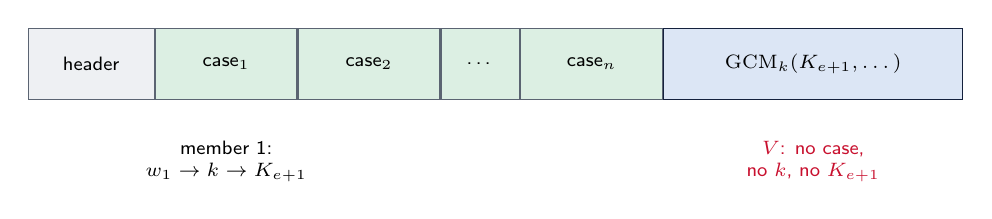
\begin{tikzpicture}[font=\scriptsize]
  \node[draw=muted, fill=hdr, minimum height=9mm, minimum width=16mm] (h) {header};
  \node[draw=muted, fill=rel, minimum height=9mm, minimum width=18mm, right=0pt of h] (c1) {case$_1$};
  \node[draw=muted, fill=rel, minimum height=9mm, minimum width=18mm, right=0pt of c1] (c2) {case$_2$};
  \node[draw=muted, fill=rel, minimum height=9mm, minimum width=10mm, right=0pt of c2] (cd) {\dots};
  \node[draw=muted, fill=rel, minimum height=9mm, minimum width=18mm, right=0pt of cd] (cn) {case$_n$};
  \node[draw=navy, fill=scr, minimum height=9mm, minimum width=38mm, right=0pt of cn] (bo) {$\mathrm{GCM}_k(K_{e+1},\dots)$};
  \node[below=4mm of c1, align=center] {member 1:\\$w_1\to k\to K_{e+1}$};
  \node[below=4mm of bo, align=center, text=accent] {$V$: no case,\\no $k$, no $K_{e+1}$};
\end{tikzpicture}
\vspace{7mm}
\begin{itemize}
  \item relays, $V$ included, forward the frame unchanged
  \item $V$ keeps relaying the new traffic; it cannot read it
  \item an observer can count the remaining members (one case each)
  \item wait one ANNOUNCE period (30\,s) after a join before revoking
\end{itemize}
\end{frame}

\begin{frame}{What each party learns}
{\small
\begin{tabular}{@{}lccc@{}}
\toprule
 & radio listener & relay, not a member & member \\
\midrule
addresses, hops left, time & yes & yes & yes \\
size and timing of traffic & yes & yes & yes \\
text of a group message & no & no & \textbf{yes} \\
forge or alter a message & no & no & yes \\
\bottomrule
\end{tabular}}
\vspace{6mm}
\textbf{Accepted limits of this prototype}
\begin{itemize}
  \item payload privacy, not location privacy (the Bluetooth address is stable)
  \item a non-member relay can drop, delay, or rewrite TTL
  \item an active outsider can flood junk or pre-empt a (source, sequence)
  \item a rogue member can grind its identifier to become coordinator
\end{itemize}
\end{frame}

% =====================================================================
% 21--28 min  hardware and results
% =====================================================================
\begin{frame}{Six boards, two roles}
{\small
\begin{tabular}{@{}lll@{}}
\toprule
 & Thundercomm RUBIK Pi 3 & Arduino UNO Q \\
\midrule
Role on the stand & screen & relay \\
SoC & Qualcomm QCS6490 & Qualcomm QRB2210 \\
OS, kernel & Ubuntu 24.04, 6.8 & Debian 13, 7.0 \\
BlueZ & 5.72 & 5.82 \\
Controller & BCM4345C5 (BT 5.0) & WCN399x (BT 5.1) \\
\bottomrule
\end{tabular}}
\vspace{5mm}
On this UNO Q image the controller cannot dial while it is peripheral,
so relays always dial and screens never do.
\vspace{2mm}
\centering
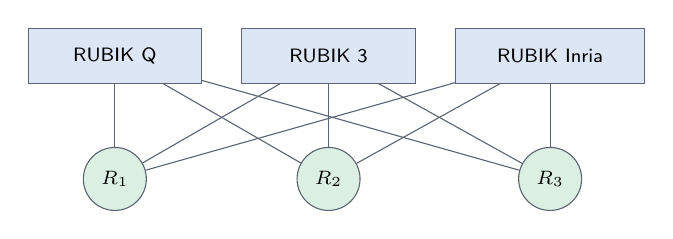
\begin{tikzpicture}[font=\scriptsize]
  \node[draw=muted, fill=scr, minimum width=22mm, minimum height=7mm] (a) {RUBIK Q};
  \node[draw=muted, fill=scr, minimum width=22mm, minimum height=7mm, right=5mm of a] (b) {RUBIK 3};
  \node[draw=muted, fill=scr, minimum width=24mm, minimum height=7mm, right=5mm of b] (c) {RUBIK Inria};
  \node[circle, draw=muted, fill=rel, minimum size=8mm, below=8mm of a] (r1) {$R_1$};
  \node[circle, draw=muted, fill=rel, minimum size=8mm, below=8mm of b] (r2) {$R_2$};
  \node[circle, draw=muted, fill=rel, minimum size=8mm, below=8mm of c] (r3) {$R_3$};
  \foreach \x in {a,b,c} \foreach \y in {r1,r2,r3} \draw[muted] (\x)--(\y);
\end{tikzpicture}
\figcap{On a table the graph is $K_{3,3}$: every message between screens
crosses a relay that is not in the group.}
\end{frame}

\begin{frame}{On the stand}
\centering
\vspace{4mm}
\metric{75/75}{receptions on the five\\other boards}
\hfill
\metric{4.4 s}{rebooted screen reads\\the group after daemon start}
\hfill
\metric{130 s}{cut controller reads again,\\no reboot of the board}
\vspace{10mm}

\metric{427/429}{six-node manual soak\\(first and last lost)}
\hfill
\metric{no}{revoked board reads\\the next message (2/2)}
\hfill
\metric{10 / 30}{sustained msg/s\\UNO Q / RUBIK}
\vspace{8mm}
\figcap{AES-GCM is 30k--173k pkt/s. Above 10\,msg/s the UNO Q runs out of
L2CAP signalling identifiers --- a kernel leak, not the crypto.}
\end{frame}

\begin{frame}{Four hops across a building}
Boards about 15\,m apart, one relay off, on battery.\\
The mesh formed a line by itself. On-board logs; clocks within 50\,ms.
\vspace{3mm}
\centering
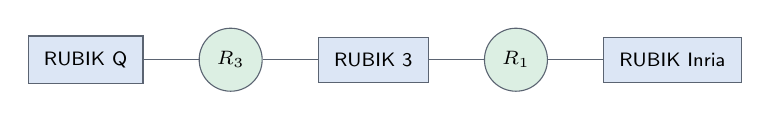
\begin{tikzpicture}[font=\scriptsize]
  \node[draw=muted, fill=scr, inner sep=2mm] (a) {RUBIK Q};
  \node[circle, draw=muted, fill=rel, minimum size=8mm, right=7mm of a] (b) {$R_3$};
  \node[draw=muted, fill=scr, inner sep=2mm, right=7mm of b] (c) {RUBIK 3};
  \node[circle, draw=muted, fill=rel, minimum size=8mm, right=7mm of c] (d) {$R_1$};
  \node[draw=muted, fill=scr, inner sep=2mm, right=7mm of d] (e) {RUBIK Inria};
  \foreach \u/\v in {a/b,b/c,c/d,d/e} \draw[muted] (\u)--(\v);
\end{tikzpicture}
\vspace{2mm}
\begin{columns}[T,onlytextwidth]
\begin{column}{0.55\textwidth}
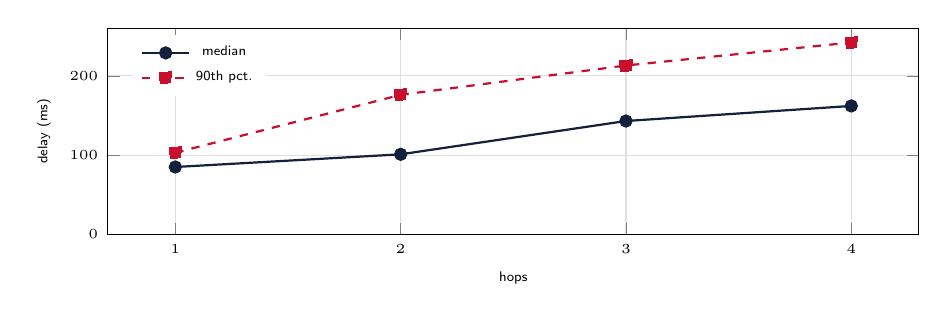
\begin{tikzpicture}
\begin{axis}[width=0.98\linewidth, height=42mm,
  xlabel={hops}, ylabel={delay (ms)},
  xmin=0.7, xmax=4.3, ymin=0, ymax=260, xtick={1,2,3,4},
  legend pos=north west, legend style={font=\tiny, draw=none},
  grid=major, grid style={gray!25}, tick label style={font=\tiny},
  label style={font=\tiny}]
\addplot[thick, mark=*, navy] coordinates {(1,85) (2,101) (3,143) (4,162)};
\addlegendentry{median}
\addplot[thick, dashed, mark=square*, accent] coordinates {(1,103) (2,176) (3,213) (4,242)};
\addlegendentry{90th pct.}
\end{axis}
\end{tikzpicture}
\end{column}
\begin{column}{0.43\textwidth}
\begin{itemize}
  \item far end: \textbf{76/79}
  \item the three misses: line still forming
  \item last link held to $\sim$30\,m
  \item sender's only relay unplugged: \textbf{95 s} dark
\end{itemize}
{\scriptsize\color{muted}A line has no detour. Mobility looked like ordinary link churn.}
\end{column}
\end{columns}
\end{frame}

\begin{frame}{8.2 hours on one charge}
Stand on battery, one message every 30\,s from RUBIK Q.\\
988 messages, 4\,915 expected receptions. We stopped the run; the batteries were not empty.
\vspace{2mm}
\centering
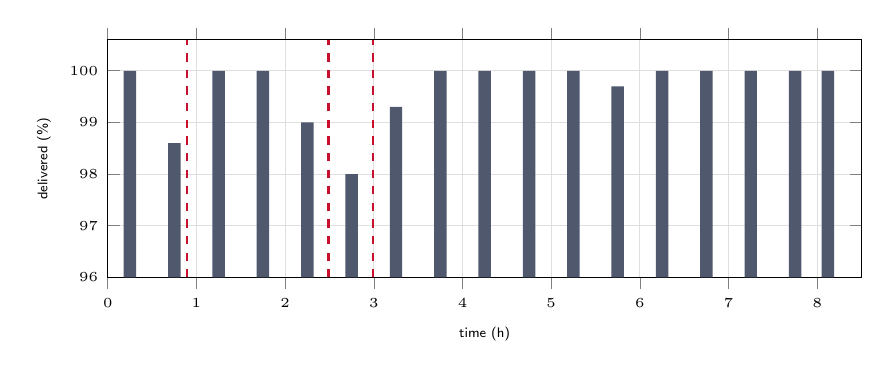
\begin{tikzpicture}
\begin{axis}[width=0.92\linewidth, height=46mm,
  xlabel={time (h)}, ylabel={delivered (\%)},
  xmin=0, xmax=8.5, ymin=96, ymax=100.6,
  xtick={0,1,...,8}, ytick={96,97,98,99,100},
  ybar, bar width=4.5pt, bar shift=0pt,
  grid=major, grid style={gray!25},
  tick label style={font=\tiny}, label style={font=\tiny}]
\addplot[fill=navy!75, draw=none] coordinates {
  (0.25,100) (0.75,98.6) (1.25,100) (1.75,100)
  (2.25,99.0) (2.75,98.0) (3.25,99.3) (3.75,100)
  (4.25,100) (4.75,100) (5.25,100) (5.75,99.7)
  (6.25,100) (6.75,100) (7.25,100) (7.75,100) (8.12,100)};
\draw[accent, dashed, thick] (axis cs:0.89,96) -- (axis cs:0.89,100.6);
\draw[accent, dashed, thick] (axis cs:2.49,96) -- (axis cs:2.49,100.6);
\draw[accent, dashed, thick] (axis cs:2.99,96) -- (axis cs:2.99,100.6);
\end{axis}
\end{tikzpicture}
\figcap{Dashed: controller reloads on two UNO Q relays (about two minutes deaf,
no reboot). Screens 100\%, relays 99.3\%. Median 80\,ms, 99th percentile 188\,ms. 6/6 still up.}
\end{frame}

\begin{frame}{Three defects, found by measuring}
\begin{enumerate}
  \item \textbf{Shared anti-replay window.} ANNOUNCE and data used one
        window: a data frame with an ANNOUNCE's sequence was dropped
        everywhere. \emph{Fixed, regression test.}
  \item \textbf{Split-brain coordinator.} On a sparse 30-node graph, four
        nodes elected themselves. \emph{Fixed: one membership view,
        regression test.}
  \item \textbf{Sequence numbers die on restart.} After the sender's
        daemon restarted, every receiver's window silently dropped it.
        Only a receiver restarted afterwards accepted the new messages.
        \emph{Open: sequence numbers must survive a restart.}
\end{enumerate}
\vspace{3mm}
{\color{muted}\small Defect 3 appeared at the end of the 8.2\,h run, when the
sender daemon was restarted on the measuring laptop.}
\end{frame}

\begin{frame}{TTL is a hop budget, not a node count}
Shipped forwarder, random geometric graphs, three sources per draw.
\vspace{3mm}
\centering
{\small
\begin{tabular}{@{}rrrrr@{}}
\toprule
nodes & degree & eccentricity & min TTL & delivery @ TTL 10 \\
\midrule
10 & 3.9 & 4 & 4 & 100\% \\
20 & 4.3 & 8 & 8 & 100\% \\
30 & 3.3 & 11 & 11 & 93\% \\
50 & 5.2 & 13 & 13 & 94\% \\
100 & 5.2 & 19 & 19 & 23\% \\
\bottomrule
\end{tabular}}
\vspace{5mm}
The minimum TTL that reaches everyone equals the worst source's
eccentricity, on every draw.\\
Revocation, $n=6$ to $30$: no stranded member, no leak to the excluded one.
\end{frame}

\begin{frame}{From a stand to a contact graph}
Every board already logs every link change with a timestamp.
\vspace{5mm}
That log \textbf{is} a contact graph.
\vspace{4mm}
\begin{itemize}
  \item the unit-disk simulations can be replayed on real traces
  \item then we can see how CDS election and revocation behave when
        \emph{people} move, not boards on a table
  \item the four-hop walk already looked like ordinary link churn
\end{itemize}
\vspace{5mm}
{\color{muted}\small Also open: an Android port of the CoC transport, and the
energy of AES-GCM versus the radio.}
\end{frame}

% =====================================================================
% close
% =====================================================================
\begin{frame}{What to try on the stand}
Three RUBIK Pi 3 screens, three UNO Q relays.
\vspace{5mm}
\begin{enumerate}
  \item \textbf{Send} from one screen: the message crosses a relay that
        is not in the group.
  \item \textbf{Exclude} a screen or a relay: it keeps relaying; the next
        message no longer appears on it.
  \item \textbf{Restart} the mesh: watch the links and the group come back.
\end{enumerate}
\end{frame}

\begin{frame}{Takeaways}
\begin{enumerate}
  \item An open BLE mesh with private groups is implementable without pairing.
  \item Relays read a 26-byte header. Members share $K_e$ for the group,
        and $K_{AB}$ for traffic the rest of the group must not see.
  \item Revocation is one signed flood, wrapped under those pairwise keys.
  \item On six boards: 75/75 in the room, 76/79 at four hops, 8.2\,h on
        battery at 99.7\% of deliveries.
  \item The limit we hit is the BlueZ stack of the UNO Q, and a sequence
        counter that must survive a restart.
\end{enumerate}
\end{frame}

\begin{frame}[plain]
\begin{tikzpicture}[remember picture, overlay]
  \fill[navy] (current page.south west) rectangle (current page.north east);
  \fill[accent] ([yshift=11mm]current page.south west) rectangle ([yshift=12.2mm]current page.south east);
\end{tikzpicture}
\vspace{14mm}
{\color{white}\bfseries\Huge Thank you\par}
\vspace{8mm}
{\color{white!85}Poster and stand are next door.\\
arXiv:2509.00967\par}
\vspace{10mm}
{\color{white!65}Boards provided by the Qualcomm University Platforms program.\\
paul-maxence.baraton@inria.fr}
\end{frame}

% =====================================================================
% backup
% =====================================================================
\appendix
\begin{frame}{Backup: joining, four clocks}
A new node is not ``in the group'' the moment it appears.
\begin{enumerate}
  \item presence: one advertising interval
  \item channel: one L2CAP handshake
  \item HELLO: it enters neighbours' tables
  \item ANNOUNCE ($\le$30\,s): its public keys reach beyond one hop
\end{enumerate}
\vspace{4mm}
Only after (4) can it be revoked safely.\\
The screens therefore show \textbf{link state} and \textbf{group state} separately.
\end{frame}

\begin{frame}{Backup: why the graph is $K_{3,3}$}
\begin{itemize}
  \item two screens never dial each other
  \item two UNO Qs cannot: the controller cannot dial while it is
        peripheral on any link
  \item so every path alternates screen and relay
\end{itemize}
\vspace{4mm}
The same UNO Q kernel leaks one L2CAP signalling identifier per received
credit (upstream fix: \texttt{6e1930ece855}).\\
Links are recycled before the pool of 254 runs out.\\
A watchdog reloads a controller that stops answering, without rebooting
the board.
\end{frame}

\begin{frame}{Backup: Bridgefy and the crowd}
Albrecht et al., CT-RSA 2021, on Bridgefy in large-scale protests:
\begin{itemize}
  \item impersonation
  \item tracking
  \item denial of service
\end{itemize}
\vspace{4mm}
A mesh used in a crowd must withstand those.\\
BUBBLE-BLUE answers impersonation of \emph{payloads} (GCM + signatures).\\
It does \textbf{not} answer tracking: the Bluetooth address is stable on
purpose, so a neighbour can be redialled without a bond.
\end{frame}

\end{document}
